\documentclass[tikz,border=10pt]{standalone}
\usetikzlibrary{arrows.meta,positioning,shapes.geometric,fit,backgrounds}
\begin{document}
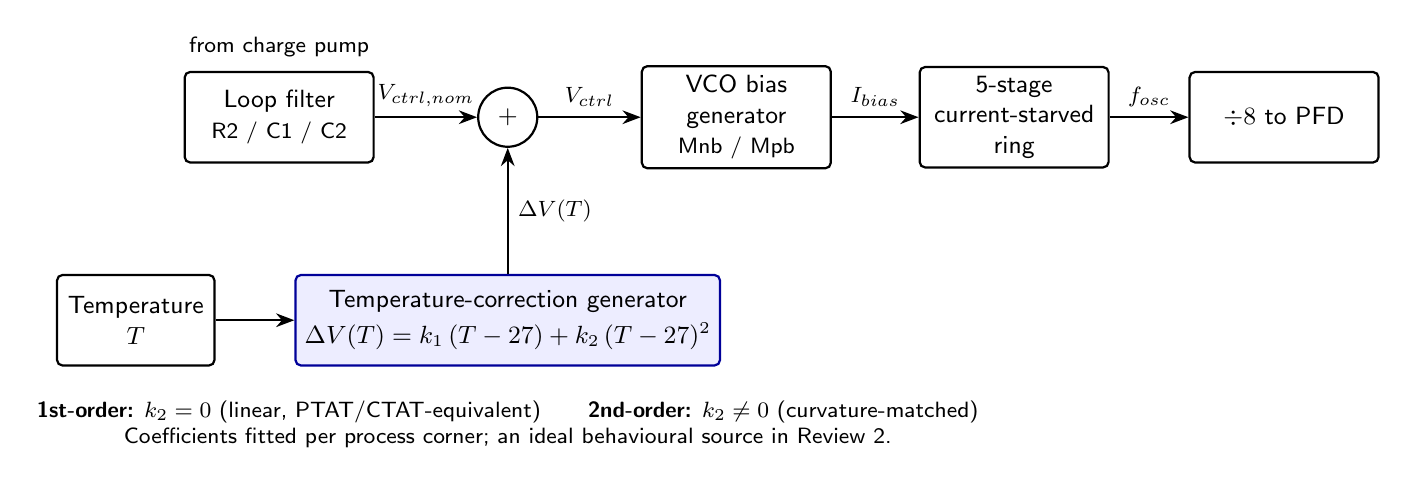
\begin{tikzpicture}[
  >=Stealth, thick, font=\sffamily\small,
  blk/.style={draw, rounded corners=2pt, minimum height=1.15cm, minimum width=2.4cm, align=center, fill=white},
  hl/.style={blk, fill=blue!7, draw=blue!60!black},
  sum/.style={draw, circle, inner sep=1.5pt, minimum size=0.75cm, fill=white},
  lab/.style={font=\sffamily\footnotesize, align=center}
]
\node[blk] (lf) {Loop filter\\{\footnotesize R2 / C1 / C2}};
\node[lab, above=0.05cm of lf] {from charge pump};
\node[sum, right=1.3cm of lf] (s) {$+$};
\node[blk, right=1.3cm of s] (bias) {VCO bias\\generator\\{\footnotesize Mnb / Mpb}};
\node[blk, right=1.1cm of bias] (ring) {5-stage\\current-starved\\ring};
\node[blk, right=1.0cm of ring] (div) {$\div 8$ to PFD};

\node[hl, below=1.6cm of s, minimum width=5.2cm] (corr) {Temperature-correction generator\\[2pt]
  $\Delta V(T) = k_1\,(T-27) + k_2\,(T-27)^2$};
\node[blk, left=1.0cm of corr, minimum width=2.0cm] (sens) {Temperature\\$T$};

\draw[->] (lf) -- node[above,lab]{$V_{ctrl,nom}$} (s);
\draw[->] (s) -- node[above,lab]{$V_{ctrl}$} (bias);
\draw[->] (bias) -- node[above,lab]{$I_{bias}$} (ring);
\draw[->] (ring) -- node[above,lab]{$f_{osc}$} (div);
\draw[->] (sens) -- (corr);
\draw[->] (corr) -- node[right,lab]{$\Delta V(T)$} (s);

\node[lab, below=0.3cm of corr] {\textbf{1st-order:} $k_2=0$ (linear, PTAT/CTAT-equivalent)\qquad \textbf{2nd-order:} $k_2\neq0$ (curvature-matched)\\
Coefficients fitted per process corner; an ideal behavioural source in Review 2.};
\end{tikzpicture}
\end{document}
